\documentclass[a4paper,12pt,oneside]{report}

\usepackage{styles/tcdthesis}
\usepackage{array}
\usepackage{booktabs}
\usepackage{tabularx}

\mastersthesis
\oneandhalfspace
\leftchapter

\graphicspath{{figures/}}

\renewcommand{\thesisschool}{School of Computer Science and Statistics}
\renewcommand{\thesisuniversity}{University of Dublin, Trinity College}
\renewcommand{\thesisauthor}{Priyansh Nayak}
\renewcommand{\thesisauthorpreviousdegrees}{, B.S. in Computer Science, University of Arizona}
\renewcommand{\thesismonth}{August}
\renewcommand{\thesisyear}{2026}
\renewcommand{\thesissubmissiondate}{August 2026}
\renewcommand{\thesistitle}{Creating Novel Virtual Reality Interfaces for Teaching Computer Architecture}
\renewcommand{\thesissupervisor}{Gareth Young}
\renewcommand{\thesisdegree}{Master of Science in Computer Science}
\renewcommand{\thesisdegreestream}{ (Augmented and Virtual Reality)}
\renewcommand{\thesisdegreeabbreviation}{M.Sc.}
\renewcommand{\thesistype}{Dissertation}

\begin{document}

\pagenumbering{roman}

\thesistitlepage
\thesisdeclarationpage

\begin{thesisabstract}
This dissertation investigates whether a bounded virtual reality learning environment can support students' understanding of selected single-cycle MIPS datapath concepts as a supplementary educational tool. The project responds to a specific teaching difficulty in computer architecture: although standard diagrams and verbal explanations can introduce instruction execution, learners may still struggle to construct a coherent mental model of how values, control choices, and architectural state changes relate across the datapath. In response, the dissertation presents a VR prototype that translates instruction execution into a guided spatial walkthrough organised around six learner-facing phases: Fetch, Decode, Execute, Memory, Write-Back, and Program Counter Update. The prototype was designed as a scoped pedagogical abstraction rather than as a cycle-accurate simulator. It supports selected instructions across Learning, Practice, and Test modes and externalises otherwise hidden datapath relationships through guided spatial interaction. 

%The system is positioned as a supplement to conventional teaching materials rather than as a replacement for them.

The prototype was evaluated through a small exploratory participant study combining questionnaire responses, a post-session knowledge check, a limited repeated baseline/post-session comparison, open-ended feedback, and researcher observations. Results showed generally positive usability and perceived-learning responses, alongside recurring discomfort and interface-friction issues. Knowledge-check performance was generally strong across several targeted concepts, while the repeated comparison showed stronger descriptive performance on some items following the overall learning session. These differences cannot be attributed to VR alone because participants received a tailored refresher before entering the headset. Observations also indicated initial progression from guided to reduced-support use while identifying continuing difficulties around controls, text burden, and selected instruction-stage decisions.

The findings suggest that the prototype shows promise as a supplementary means of making selected computer architecture concepts more tangible and easier to follow, while remaining limited by the exploratory study design, participant comfort, interface readability, and narrow instructional scope. The dissertation's main contribution is the development and evaluation of a pedagogical translation of single-cycle datapath reasoning into a sequential, learner-facing VR experience.
\end{thesisabstract}

\begin{thesisacknowledgments}
Acknowledgments to be written.
\end{thesisacknowledgments}

\tableofcontents
\listoftables
\listoffigures

\clearpage
\pagenumbering{arabic}

\chapter{Introduction}

Computer architecture is not usually difficult because students cannot name the parts of a datapath. The harder step is following what those parts are doing together. Registers, control signals, ALU behaviour, memory access, and program-counter updates are often introduced through diagrams, tables, and short instruction traces. Those materials are useful, but they do not always make the movement of data or the order of decisions easy to follow. A student may recognise the register file, the ALU, and the memory blocks while still being unsure about what is happening during the execution of a particular instruction.

This project grew out of that problem. During repeated exposure to undergraduate Computer Organization teaching, the same kinds of confusion appeared again and again. Students often found it difficult to treat the datapath as a process rather than as a picture. They mixed up register values, memory contents, and memory addresses. They could sometimes repeat a worked example, but had more trouble explaining why a value moved in one direction rather than another, or why one control choice led to a different final state. In practice, the most useful explanation was often the simplest one: draw over the datapath and walk through the instruction step by step.

The dissertation therefore explores a focused virtual reality learning environment for single-cycle MIPS instruction execution. The system is not intended to replace lectures, diagrams, or conventional simulators. It is intended as a supplementary tool that gives learners another way to work through instruction flow, value movement, and state change. The prototype organises the experience around Instruction Fetch, Instruction Decode, Execute, Memory Access, Write-Back, and PC Update, and asks the learner to work through supported instructions inside that structure.

The scope is deliberately narrow. The prototype does not try to cover the whole of computer architecture, and it is not presented as a cycle-accurate simulator. It concentrates on a selected set of single-cycle MIPS instructions and on a bounded set of learning tasks: decoding the instruction, selecting the right operands, following the path of execution, making control-related choices, and reasoning about the resulting architectural state. To support different stages of learning, the environment provides three modes, Learning, Practice, and Test, which reduce guidance over time while keeping the same overall lesson flow.

\section{Research Question and Scope}

Within that bounded scope, the dissertation is guided by the following research question:

\begin{quote}
\textit{To what extent does an immersive virtual reality-based learning environment improve students' understanding of abstract computer architecture concepts compared to traditional teaching methods?}
\end{quote}

The wording is intentionally cautious. The aim is not to argue that virtual reality is broadly superior to other teaching methods. The aim is to examine whether this particular prototype, used in this particular teaching context, offers enough educational value to justify the design and the study. For that reason, the evaluation is treated as exploratory and formative rather than as a final controlled proof of superiority over traditional approaches.

\section{Structure of the Dissertation}

The remainder of the dissertation is structured as follows. Chapter 2 places the project in context by reviewing the relevant background and related work, with particular attention to computer architecture learning, virtual reality in computer science education, and the design constraints that shape educational VR systems. Chapter 3 explains the design of the learning environment, including the learning outcomes, pedagogical choices, environment structure, and major abstractions used to make datapath behaviour teachable in VR. Chapter 4 describes how the system was implemented. Chapter 5 sets out the methodology used for the participant study, including the procedure, instruments, and ethical boundaries. Chapter 6 presents and discusses the results. Chapter 7 concludes the dissertation and identifies directions for future work.

\chapter{Background and Related Work}

The previous chapter introduced the project and its scope. This chapter provides the background needed to place that work in context. It begins with the learning problem that motivates the dissertation, then turns to interactive and immersive work in computer architecture and computer science education, and finally draws out the constraints and gaps that shaped the present project.

\section{Computer Architecture as a Learning Problem}

Computer architecture asks students to reason about a machine whose most important behaviour is hidden. A learner is expected to understand how instruction fields are decoded, how register values are selected, how the ALU is used for different classes of instruction, how memory is addressed, and how the program counter is updated. None of that is impossible to explain on paper, but it does place a heavy burden on the learner. Static diagrams show structure. Short traces show examples. The missing piece is often the transition between the two: how a flat picture becomes a moving process.

This problem is well known in practice. Architecture courses ask students to connect several kinds of representation at once: assembly syntax, instruction fields, datapath diagrams, register state, memory state, and control behaviour over time. Many students can solve a problem after seeing a worked example, but still struggle to explain why a branch changes the next program counter, why a load writes back a different value source from an arithmetic instruction, or why a sign-extended immediate matters at all. \citet{tlili2016improving} describe architecture as a subject that learners can find difficult and unmotivating under conventional classroom presentation. That diagnosis matches the teaching problem that motivated the current project.

The present dissertation focuses on a deliberately limited part of this wider area: instruction execution in a single-cycle MIPS datapath. That scope does not cover all of architecture, but it is large enough to expose the main difficulties that matter here. A learner still has to decode the instruction, identify source and destination registers, select operands, follow value flow through the datapath, and predict the resulting architectural state. The scope is therefore narrow enough to build and study within a Master's dissertation, while still being rich enough to raise the central educational questions.

\begin{figure}[htb]
\centering
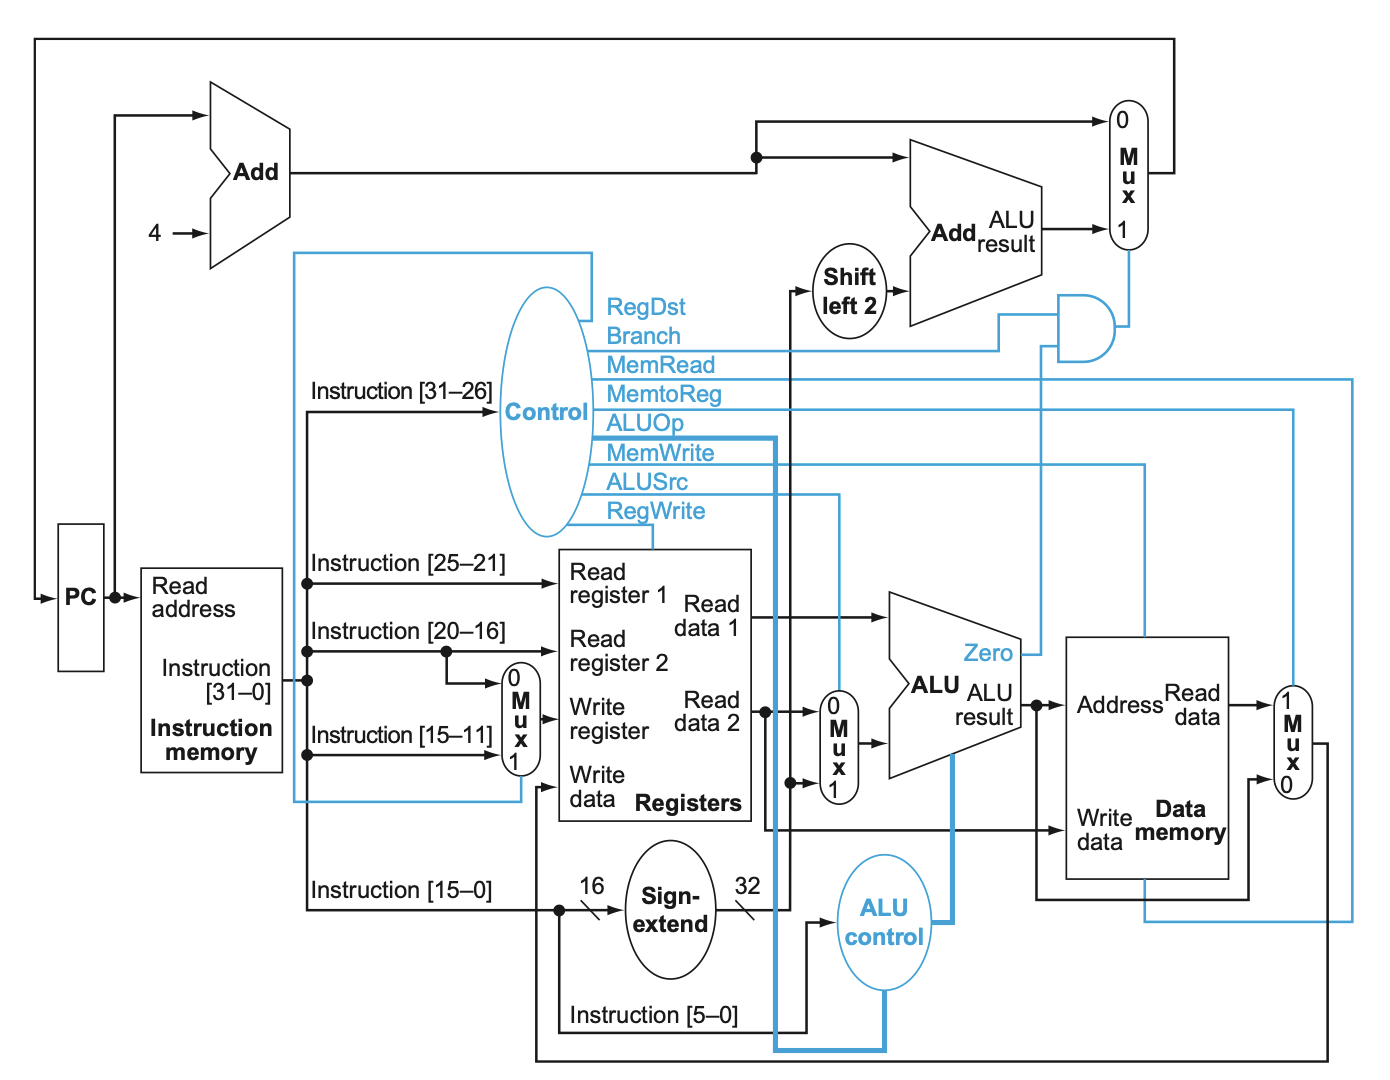
\includegraphics[width=0.9\linewidth]{datapath single cycle.png}
\captionsetup{width=.9\linewidth}
\caption[Reference single-cycle MIPS datapath]{Datapath overview attributed to Jyotiprakash Mishra's blog post on the MIPS single-cycle datapath \citep{mishraMipsSingleCycleDatapath}.}
\label{fig:referenceSingleCycleDatapath}
\end{figure}

\section{Traditional Teaching and Its Limits}

The problem described in the previous section does not mean that conventional teaching is ineffective. In most programmes, computer architecture is taught progressively rather than all at once. Basic logic is introduced first, then gates, then combinations such as half adders and full adders, then larger datapath components, and only after that does the learner meet the processor as an integrated system. Trinity College Dublin's Computer Architecture I module reflects that pattern directly through its sequence of digital logic, register transfer language, ALU and shifter design, multiplexer and tristate buses, datapath design, and the instruction fetch-decode-execute cycle \citep{tcdComputerArchitectureI}. That kind of staged build-up matters, and the present dissertation does not argue against it.

Traditional tools also do several things very well. Lectures and tutorials give a structured order in which ideas can be introduced. Whiteboard derivations are good for slowing a problem down and showing how each step follows from the previous one. Static datapath diagrams are strong at showing structure, naming components, and fixing the shape of the machine in the learner's mind. Simulators and assembly tools are good for correctness, inspection, and repeated practice. They let students test programs, inspect registers and memory, and connect assembly syntax to machine behaviour in a more formal way than a verbal explanation alone.

These strengths are important because the present project depends on them. A learner cannot make sensible use of the VR environment without some prior exposure to the underlying architectural ideas. The VR prototype is not intended to replace the gradual conceptual build-up provided by lectures, diagrams, exercises, and conventional tools. It is intended to sit alongside them, especially at the point where a student has seen the structure of the datapath but still struggles to turn that structure into a working mental model of execution flow.

The limitation of conventional teaching is therefore narrower than a simple claim that the tools are ineffective. The issue is that some of the most useful traditional materials are strongest either at showing structure or at checking correctness. They are sometimes weaker at first-pass mental-model building for learners who need to see how information moves through the machine as a sequence of linked decisions. A datapath diagram can show where the ALU sits, and a simulator can show that a register changed, but for some students the connection between those two facts is not immediate. That gap is where a supplementary spatial tool may be useful.

\section{Interactive Support for Computer Architecture Learning}

Before focusing on VR, it is worth noting that architecture learning has already been explored through other interactive formats. \citet{tlili2016improving} present an educational mobile game for computer architecture and report that learners found the approach motivating and were willing to use it again. That work is not immersive, but it matters for two reasons. First, it suggests that the subject does respond well to interactive presentation. Second, it shows that the core issue is not VR by itself. The more basic issue is how to make abstract system behaviour easier to follow.

More directly related work appears in immersive and experiential systems. \citet{dascalu2017experiential} describe a VR environment for studying computer architecture through experiential learning. Their system asks the learner to assemble virtual computer components while receiving textual guidance. The emphasis is not identical to the present project, but the paper is still important because it treats computer architecture as a credible target for immersive learning rather than as a niche or novelty application. It also shows an early attempt to move architecture teaching away from passive explanation and toward structured activity inside a virtual environment.

\citet{tan2023vr} are closer still. Their VR serious game is explicitly aimed at the Computer Organisation and Architecture subject and focuses on CPU procedures that students often find hard to visualise in conventional teaching. They report positive learning efficiency together with an engaging experience. For the present dissertation, the main value of this paper is not merely that it uses VR, but that it treats architecture learning as a sequence of actions that can be staged and guided inside a game-like structure. That is close in spirit to the current prototype, even though the present work narrows the scope more tightly around instruction execution in a single-cycle datapath.

\citet{alnuaimi2025vr} study a VR environment for digital design and computer organisation laboratory learning. Their paper is useful partly because it remains close to the broader hardware-and-systems teaching space, and partly because it keeps usability in view throughout the evaluation. Their results point to a familiar lesson: even a promising educational VR system has to be learnable and comfortable enough to use before any learning claim can matter. For the present project, that is an important reminder. A tool intended to support understanding of hidden processes can just as easily create another layer of confusion if the interface is awkward or overloaded.

\section{Virtual Reality in Computer Science Education}

The broader computer science education literature gives a clearer sense of where architecture fits within immersive teaching work. \citet{pirker2020virtual} review VR in computer science education and note its promise for areas where abstract concepts benefit from interactive visualisation. \citet{agbo2021application} reach a similar conclusion from a larger bibliometric and content review, showing that VR has been explored across a range of computer science topics and that interest in the area has grown over time. \citet{janani2026virtual} provide the most recent scoping review and show that many VR applications in computer science education are directed toward conceptual learning rather than toward full practical programming tasks.

That pattern matters here. The present dissertation is not trying to teach learners how to write larger assembly programs or reason about the whole of digital logic design inside a headset. It is concerned with conceptual understanding of instruction execution. The wider reviews suggest that this is exactly the sort of problem for which VR is most often proposed: an abstract process, difficult to observe directly, that may become easier to follow when it is made spatial, interactive, and staged.

The more specific studies within that wider literature also point in the same direction. \citet{pirker2021potential} compare VR and desktop learning for sorting algorithms and report stronger subjective measures such as presence, absorption, and positive emotion in the VR condition. \citet{mohamad2023immersive} report positive results from a mobile VR application for learning Python coding. Neither paper is about architecture, but both are relevant because they treat VR as a way of making abstract computing concepts more concrete. They also show a recurring pattern in this literature: VR is often used less to replace existing formal tools than to provide a clearer first encounter with an otherwise difficult idea.

The same reviews also point to the limits of the field. \citet{janani2026virtual} note recurring usability issues, weak collaborative features, and a lack of clear instructional grounding in parts of the literature. \citet{agbo2021application} show that much of the work is still scattered across topics and methods. This is useful context for the present dissertation. It suggests that a contribution does not need to claim that VR in CS education is entirely new. The more realistic contribution is to show a careful application in a domain where the match between problem and medium is strong.

\section{Design Constraints and Transferable Lessons}

The case for VR is therefore not enough on its own. The next question is what kind of VR design is likely to help rather than hinder. \citet{cook2019challenges} discuss educational VR in terms of practical constraints as much as opportunity. Their work draws attention to issues such as deployment, accessibility, sustainability, and the amount of support institutions need before VR becomes a normal teaching tool. For a dissertation-scale prototype, this is a useful corrective. It shifts the emphasis away from spectacle and toward a more modest question: can a system be clear, usable, and worth the time required to use it?

\citet{korkut2023visualization} approach a related problem from the perspective of VR visualisation. They point out that immersive space does not automatically solve information-design problems. Poor layout, visual clutter, and badly organised interaction can still make a system hard to read. That lesson carries directly into architecture teaching, where the central challenge is already one of representing a hidden process without losing the learner in detail. If too much of the datapath is surfaced at once, VR may reproduce the original problem in another form.

\citet{samala2025virtual} make a similar point at the level of educational trends. Their review shows continuing interest in VR across education, but also repeated concerns about readiness, hardware access, discomfort, and the quality of actual learning design. This is helpful for keeping the present dissertation honest. A small architecture-learning prototype does not need to solve the institutional adoption problem, but it does need to avoid assuming that immersion alone will produce learning.

Some of the more transferable papers in the reading set sharpen this issue further by looking at abstract visualisation outside architecture. \citet{lee2020data} argue that VR can support deeper intuitive understanding when information is mapped in a way that users can feel and navigate, but they also warn that complexity can weaken focus. Work by Oberhauser \citep{oberhauser2018database,oberhauser2019database} and \citet{kellmann2024visualization} on database and linked-data visualisation is not about architecture, but it still matters because it shows that VR can be used to represent non-physical structures in ways that support navigation and comprehension. That lesson transfers well to the present project. A datapath is not a physical space that a learner can enter, but it can be turned into a navigable structure if the transformation is done carefully.

\section{Implications for the Present Project}

Several design implications follow from this literature. First, the case for using VR in computer architecture does not rest on novelty. It rests on a specific match between medium and problem: hidden, dynamic behaviour that learners often struggle to reconstruct from a static diagram. Second, the most useful systems are not simply more immersive versions of existing teaching material. They are selective. They decide what to externalise, what to keep simple, and where the learner should act rather than only observe.

Third, architecture learning seems to benefit from guidance and progression. This appears in game-based work such as Tlili et al. \citep{tlili2016improving} and Tan et al. \citep{tan2023vr}, and it also appears indirectly in the broader CS-education literature where prompts, panels, and staged activities are common design patterns \citep{janani2026virtual}. For the present dissertation, that supports the use of Learning, Practice, and Test as a progression rather than as three unrelated modes.

Fourth, the literature repeatedly warns against overload. A datapath can be made more visible in VR, but that does not mean every hidden detail should be turned into an explicit interaction. \citet{cook2019challenges}, \citet{korkut2023visualization}, \citet{samala2025virtual}, and \citet{lee2020data} all point in the same direction: if the learner is asked to manage too many objects, too much text, or too much movement at once, the value of the medium starts to disappear.

The gap addressed by the present project can therefore be stated fairly plainly. There is already evidence that interactive and immersive approaches can support computer architecture learning, and there is a broader body of work showing that VR can help with abstract computer science concepts. What remains less well served is a tightly scoped learning environment centred on manual instruction tracing through a single-cycle datapath, with explicit attention to operand selection, stage-by-stage decisions, and the final architectural state. That is the niche occupied by the current prototype. The next chapter explains how the design of that prototype was shaped by the literature reviewed here and by the teaching problem set out in Chapter 1.

\section{Summary}

The literature does not justify an argument that VR is automatically good for education, or even automatically good for computer architecture. It does justify a narrower claim. Computer architecture is a strong candidate for interactive support because much of the subject depends on understanding dynamic processes that are hard to see directly. Existing work shows that architecture learning has already been explored through mobile games, experiential environments, and VR serious games, while the wider VR-in-CS-education literature shows that conceptual learning is one of the medium's more plausible uses. The same literature also sets clear limits: guidance matters, usability matters, and information must be presented with restraint. Those are the conditions under which the present dissertation takes shape.

\chapter{Methodology}

This chapter sets out the method used to evaluate the prototype. The study was conceived as a small-scale exploratory evaluation of a deliberately scoped educational system; it was not designed as a controlled comparison or as a test of whether VR should replace conventional teaching.

\section{Research Framing}

The evaluation considered whether the prototype was educationally useful within its intended scope, whether participants could engage with it clearly enough for that value to matter, and whether the combined evidence justified further development for selected computer architecture concepts.

As noted in Chapter~1, the prototype grew out of repeated teaching-assistant experience in computer organisation. The study therefore examined whether the guided tracing that proved useful in that setting could be translated into a useful VR-based learning environment, a question that also sits in line with earlier architecture-focused immersive work \cite{dascalu2017experiential,tan2023vr}.

\subsection{Research Question}

The dissertation was guided by the following research question:

\begin{quote}
\textit{To what extent can an immersive virtual reality learning environment support students' understanding of selected single-cycle MIPS datapath concepts as a supplementary educational tool?}
\end{quote}

In this dissertation, the phrase ``to what extent'' is to be interpreted in a bounded exploratory sense rather than as a promise of a full classroom control-group comparison. More specifically, the question is answered through three linked forms of evidence: participant perceptions of the environment, descriptive concept evidence drawn from the baseline subset and post-session responses, and observed progression or support needs across the session structure.

The purpose of the study was therefore to determine whether this particular prototype, used in this particular educational context, offered enough conceptual clarity, usability, and perceived value to justify the design choices behind it and support later work on broader evaluation.

\subsection{Evaluation Aspects}

The research question was examined through four linked evaluation aspects reflecting the prototype's intended educational role:

\begin{enumerate}
\item \textbf{Usability and clarity.} Whether participants could understand, navigate, and use the system clearly enough for its educational purpose to be evaluated.
\item \textbf{Conceptual support.} Whether the collected evidence suggested that the environment helped participants follow instruction flow, datapath phases, component roles, and selected architectural relationships.
\item \textbf{Progression from guided to reduced support.} Whether participants could move from the guided structure of Learning mode into less-supported interaction in Practice or Test mode, and what support remained necessary during that transition.
\item \textbf{Supplementary educational value.} How participants perceived the prototype in relation to lectures, diagrams, tutorials, simulators, and other conventional teaching materials.
\end{enumerate}

\section{Alignment with the Learning Outcomes}

The evaluation was aligned with the learning outcomes defined for the prototype, but those outcomes belong primarily to the design of the system and are discussed in full in Section~4.1. In methodological terms, they matter here because they establish what the study should look for and what kinds of claims the evidence can reasonably support.

The study therefore focused on a bounded cluster of educational tasks: decoding supported instructions, explaining the roles of major datapath components, tracing instruction and value flow across the main lesson phases, making the required operand and control-facing choices, predicting resulting architectural state changes, reasoning across different supported instruction classes, and completing the walkthrough with progressively less support. These categories were reflected across the baseline subset, the post-session knowledge check, the observation notes, and the broader interpretation of participant feedback.

\section{Study Design and Participants}

Structured evidence came from the background form, the baseline subset, the Likert-style post-session items addressing perceptions of the system, and the knowledge check on selected concepts. Open-ended evidence came from written participant feedback and researcher observation notes recorded during and after the session. These sources were considered together to provide a fuller account of how the prototype functioned as a learning tool.

The evaluation remained exploratory rather than classroom-trial in scale. There was no formal non-VR control group and the study did not attempt to measure long-term retention. The design instead focused on how participants engaged with the prototype and whether the collected evidence supported its intended role as a supplementary learning environment, consistent with broader literature on conceptual VR support in computer science education \cite{janani2026virtual,dengel2020important}.

Twelve participants took part in the completed study through voluntary convenience sampling. All participants were consenting adults aged 18 or over. The approved ethics application had initially set a target sample size of twenty participants, while the completed recruitment yielded twelve. Recruitment took place by email invitation, no payment was offered, and the study involved no dependent relationship between the research team and participants. Background information on prior architecture exposure, prior VR use, confidence, and topic familiarity was collected before the session so that the findings could be interpreted in light of participants' different starting points; these characteristics are reported in Chapter~6.

\section{Procedure}

Each participant session followed the same broad structure: consent and background capture, a short baseline probe, a tailored refresher, the VR session itself, and a post-session evaluation.

The session began with the Participant Information Leaflet and written informed consent, both of which are reproduced in Appendix~\ref{app:pil} and Appendix~\ref{app:consent} respectively. Participants were given the opportunity to read the study information, ask questions, and decide whether they wished to continue before any data collection began. They then completed the background section of the questionnaire reproduced in Appendix~\ref{app:questionnaire}, which captured prior VR use, prior exposure to computer architecture or computer organisation, and self-reported familiarity and confidence.

After the background section, participants were offered a short baseline subset drawn from the knowledge check reproduced in Appendix~\ref{app:questionnaire}. This consisted of five pre-session questions used as a modest checkpoint on foundational ideas before the VR experience began, specifically Questions 11--14 and 25 from the post-session questionnaire in Appendix~\ref{app:questionnaire}. Because this baseline acted as a quick pre-session scan rather than a mandatory scored gate, unanswered items were retained as missing rather than treated as incorrect. Participants then received a short verbal refresher tailored to their prior experience. The refresher was intentionally high-level: it was not meant to teach the whole content in advance, but to align terminology, reduce avoidable confusion, and give participants enough orientation to engage meaningfully with the prototype. Typical coverage included the basic form of an assembly instruction, what the datapath represents, what the main instruction stages do, how registers and memory differ, where control choices matter, and what kinds of interaction participants would encounter in the VR environment.

Participants then completed the VR session using selected instructions and one or more of the available modes. A recorded walkthrough of the prototype, representative of what participants were seeing during the live study, is available at \url{https://youtu.be/Y8tFYnWeLtI}. The exact path depended on participant background, session time, and whether the participant appeared comfortable enough to move into reduced-guidance modes. A typical path included one or two Learning mode instructions, one Practice mode instruction, and, where appropriate, a further Test mode attempt. During the session, the researcher intervened only when needed, and participants were encouraged to make full use of the resources available inside the environment. The amount and kind of intervention required were themselves treated as meaningful observational data.

After removing the headset, participants completed the remaining sections of the questionnaire reproduced in Appendix~\ref{app:questionnaire}. These included Likert-style ratings on usability, engagement, and perceived learning, followed by the broader knowledge-check section and open-ended feedback. Alongside the formal questionnaire data, the researcher maintained brief session notes on participant support, attempted instructions and modes, points of hesitation, and relevant comparisons with traditional materials.

\section{Instruments and Data Capture}

The primary structured instrument was the Microsoft Forms questionnaire used in the live study. It captured participant background, post-session usability, engagement and perceived-learning responses, the targeted knowledge check and follow-up confidence item, and open-ended feedback. A reconstructed print version of the deployed questionnaire is reproduced in Appendix~\ref{app:questionnaire}, while the Participant Information Leaflet, consent form, and representative recruitment materials are reproduced in Appendix~\ref{app:pil}, Appendix~\ref{app:consent}, and Appendix~\ref{app:recruitment}.

The knowledge-check portion of the live form focused mainly on topics relevant to the implemented prototype: program-counter behaviour, fetch, the instruction register, stage order, the execute stage, branch-related reasoning, and the behaviour of supported MIPS instructions such as \texttt{add}, \texttt{addi}, \texttt{lw}, \texttt{sw}, \texttt{beq}, and \texttt{j}. A small number of surrounding architecture concepts were also retained so that responses could be interpreted against the broader background knowledge with which participants entered the session, while the main evaluative focus remained on the selected datapath concepts supported by the prototype.

Some participant-facing materials, most explicitly the Participant Information Leaflet in Appendix~\ref{app:pil}, described the study using broader computer architecture examples such as pipelining, memory hierarchy, and stack behaviour. These materials are reproduced unchanged for transparency because they formed part of the approved ethics documentation before the final prototype scope was fully settled. The evaluated VR session itself remained limited to the selected single-cycle MIPS datapath concepts defined in this dissertation.

Researcher notes supplemented the questionnaire by recording attempted instructions and modes, points of hesitation, support requirements, and relevant comparisons participants made with conventional learning materials.

\section{Analysis Plan}

The analysis was primarily descriptive and combined evidence on usability, conceptual support, participant understanding, and supplementary educational value. The small sample and exploratory design did not justify strong inferential testing, so the evidence was interpreted through descriptive statistics, item-level patterns, open-ended feedback, and researcher observations. IBM SPSS Statistics was used for quantitative analysis, while NVivo supported the organisation of qualitative material.

Quantitative analysis summarised participant background, item-level Likert responses and descriptive group measures, knowledge-check performance, post-knowledge-check confidence, and the limited baseline/post-session comparison. Frequencies, percentages, means, medians, ranges, and internal-consistency estimates were reported where appropriate to the measure being described. Baseline and post-session responses were compared descriptively only on the repeated items for which matched data were available.

Open-ended responses and researcher observation notes were read together through a light thematic analysis. The analysis focused on recurring material concerning what helped understanding, what remained confusing, interface or navigation friction, the guidance structure, and comparisons with conventional learning materials.

Because the study did not include a formal non-VR control group, comparison remained indirect and drew on participant perceptions, the limited repeated baseline/post-session items, and observed progression from guided to less-guided performance. The baseline subset was followed by a short verbal refresher before the VR session itself, so any baseline/post-session differences were interpreted as performance following the overall learning session rather than as evidence attributable to the VR environment alone.

\section{Ethical Considerations and Study Boundaries}

The study received research ethics approval through the School of Computer Science and Statistics Research Ethics Management System (REAMS). Participation was voluntary and based on informed consent, with participants receiving study information before taking part and retaining the right to withdraw without penalty. They were also informed that withdrawal of research material might no longer be possible once data had been anonymised and incorporated into the analysis.

The principal participant risk was temporary discomfort associated with VR use, including eye strain, dizziness, or motion sickness. Participants could pause or stop the session immediately if they felt unwell, and task completion was not prioritised over participant comfort.

Administrative contact information was kept separate from research responses, and research materials were anonymised as early as practicable. Access to identifiable data was restricted to what was necessary for the study, with storage limited to password-protected and university-approved systems in line with the approved data-handling plan. Identifiable or coded administrative data were retained only for a limited period before deletion.

The study used a Meta VR headset supplied through the School, and participants were not required to sign into personal Meta accounts. The research team did not intentionally collect Meta account data, although participant materials noted that limited device-level or platform-level processing outside the direct control of the research team could still occur.

\section{Use of Generative Artificial Intelligence}

In accordance with Trinity College Dublin's \textit{College Statement on Artificial Intelligence and Generative AI in Teaching, Learning, Assessment \& Research} (2024), the use of generative artificial intelligence in the development of this project and preparation of the dissertation is acknowledged below.

ChatGPT (GPT-5.6 Sol, OpenAI, \url{https://chatgpt.com}) was used in a supporting capacity to clarify selected computer-architecture concepts during development, including walkthroughs of how supported instructions operate through a single-cycle datapath. It was also used to help standardise BibTeX entries where citation information obtained from Google Scholar and individual publisher websites was inconsistent, and to provide critique and proofreading of author-written dissertation material.

Codex (GPT-5.4, OpenAI, \url{https://openai.com/codex/}) was used in a limited support capacity. Its primary use was to help maintain and organise a project journal so that implementation milestones and decisions could later be referred back to as historical summaries. It also provided limited assistance with repository organisation, the Python data-processing pipeline used to clean, restructure, and prepare collected study data for analysis, and the preparation of tables. Codex was not used to create, fabricate, invent, simulate, or alter participant data, results, or findings.

\section{Summary}

This chapter established the methodological framework for the exploratory evaluation, including the study design and participants, procedure, data-collection instruments, analysis strategy, and ethical considerations. The analysis remained primarily descriptive, while the tailored refresher between the baseline probe and VR session means that any baseline/post-session differences reflect the overall learning session rather than an effect attributable to VR alone. Chapter~4 turns from this methodological framework to the design decisions through which the targeted datapath concepts were translated into a guided, learner-facing VR environment.
\chapter{Design}

\section{Design Goals}

\textit{What should go here:} restate the specific teaching problem the design responds to. Connect the chapter back to the methodology by showing that the design exists to address the stated learning outcomes and hypotheses rather than to showcase VR for its own sake.

\section{Learning Outcomes as Design Drivers}

\textit{What should go here:} show how each learning outcome shaped the structure of the environment. This is where the dissertation should make explicit that the prototype was scoped around supported instruction execution tasks rather than around the whole of computer architecture.

\section{Pedagogical Approach}

\textit{What should go here:} explain the teaching model behind the system. This should cover guided tracing, progressive reduction of support, the role of embodied interaction, and the decision to treat the prototype as a supplement to lectures, diagrams, whiteboard explanation, and conventional practice materials.

\section{Environment Structure}

\textit{What should go here:} describe the overall layout of the environment and the logic of the learner's movement through it. Explain why the prototype was organised as a sequence of world-space teaching stations rather than as a floating menu or a purely abstract simulator.

\section{Mode Structure}

\textit{What should go here:} explain the roles of Learning, Practice, and Test. This section should show how the three modes embody progression from explicit guidance to more independent completion while preserving a common lesson structure.

\section{Interaction Model}

\textit{What should go here:} describe the main learner actions that matter pedagogically, such as decoding, register selection, datapath progression, operand or route choice, validation, and end-state reasoning. Make clear which interactions were made physical and which were left to UI support, and why.

\section{Representational and Pedagogical Abstractions}

\textit{What should go here:} explain where the prototype stays close to the textbook single-cycle datapath and where it deliberately departs from strict hardware realism. This is the place to discuss externalised hidden processes, staged progression, physical datapackets, and the decision to preserve reasoning structure rather than literal timing.

\section{Core Design Decisions and Trade-Offs}

\textit{What should go here:} gather the important design choices in one place. This should include scope narrowing, supported instruction classes, readability versus realism, stability versus feature expansion, and the trade-off between pedagogical clarity and simulation fidelity.

\chapter{Implementation}

The purpose of this chapter is to showcase how the design was realized in the final build of the prototype that was used for conducting the research study. The system was implemented as a Unity-based Virtual Reality application centred on an authored lesson scene, a shared lesson-flow architecture, and a set of phase-specific stations corresponding to the standard MIPS single-cycle datapath, consisting of fetch, decode, execute, memory access, write-back, and a bonus program-counter update phase. The learner encounters these parts as a spatial route coordinated by a runtime structure that tracks lesson state, instruction context, progression, validation, and mode-specific behaviour.

The application is influenced by runtime instances of instruction selection, mode changes, phase activation, local feedback, and state changes, as the user progresses through the lesson. The arrangment was facilitated as such to support a complete walkthough, varied by instruction and modes, and tightened enough for assesment and allignment with the learning outcomes.

It does not attempt to reproduce the literal internal timing of a textbook or actual variant of the microprocessor, as the build intentionally selects specific hidden processos to turn into visible learner-facing actions that can dictate the flow of the datapath while being abstracted enough to not overflow the user with excessive workload or information, all the while retaining educational context.

\section{Platform and Development Context}
The prototype was developed in Unity version 6000.4.11f1 and deployed as a Virtual Reality application. Unity provided the practical combination of the world-space interaction, scene layout, an headset deployment needed for the project in the form of Unity's XR Interaction Toolkit v. 3.4.1 and OpenXR-based platform support (v. 1.16.1, meta version 2.5.0), which provided the baseline resources for XR grabbable logic, world-space UI, and general scene interactions. This project would not claim to have created these baselines projects from scratch, but instead built upon it by configuring these resources as per the task at hand.

The environment and assets were developed using free asset packs from Unity Asset Store, namely Free LowPoly Scifi pack by Cuboom \cite{cuboom2018lowpoly} and 3D Sprite Sci-Fi props by Oiva Kahri \cite{kahri2023scifi}. The asset packs were used for the creation of the various props, interactables, and overall environment scene, as well as translation of certain unique behavioural patterns such as scanning and retrieval of data from a register, updation of data memory or registers, and dictating phase-specific stations.

The technical foundations had direct consequences for the shape of the build, as it required the proper split of authored elements that would give shape to the overall structure of the datapath and the resources that would experience runtime specific manipulation. Main authored elements came in the form of phase-specific stations, phase-wise user interfaces, and various miscellanous elements such as the register bank and data memory. While the core objects were all bounds through serialized references and components, an equal chunk of resources went into the creation of runtime only behaviours and object manipulation that influenced the lesson flow directly.

\section{Overall System Architecture}

The software structure of the prototype is organized around one shared lesson runtime which coordinates the many phase-wise stations and resources distributed across the environment to keep the mode logic, instruction data, validation state, and progression behavior consistent across the experience.

The central lesson object is CpuLessonFlow.cs, which acts as the scene facing root of the lesson runtime, storing the current lesson mode, the selected instruction context, and the current step within the lesson. This is directly responsible for raising state-change and feedback evenets used by the surrounding UIs and phase controllers, thus preventing complete independence of the stations, and acting as an orchestrator that determines the type of interactions required at each step.

That shared runtime is further supported by the authored lesson guide layer called the LessonGuideController which is responsible for tying the central lesson flow to the visible lesson panels, UI interactables responsible for phase progression, and mode-specific supports. It is also responsible for coordinating the active panel and its objects set across the lesson route, to make the experience feel more sequential. In simple terms, the guide controller is the bridge between the underlying lesson state and the learner-facing instructional layer.

Then there's a LessonPhaseRouter that gives both systems a shared understanding of whih phase currently own's the learner's next action, and a LessonModePolicy which centralises the broad behavioural differences between the three distinct modes so that hint availability, scanner and validation budgets, and panel visibility remains consistent across the board.

The rest of the architecture is divided into focuses subsystems, with dedicated controllers for each major phase, as well as coordinators and individual components that handle registers, data packets, instructions, navigational guidance, gates, and also shared UI support. The architecture was properly separated into a hierarchal order, with one shared runtime, several stage-specific systems, and a support layer that keeps common behaviour consistent.

\subsection{Core Runtime Controllers}

The main runtime relationship is between the lesson-flow controller (CpuLessonFlow) which owns the lesson state and progression behaviour, the lesson-guide controller (LessonGuideController) which owns the visible instructional surfaces and their response to the flow state, and the phase controllers that own the logic and validation of their respective stations.

This division allowed the proper separation of progression and station logic, by isolating phase-specfic behaviour such as required input handling and validation without needing every individual objects to require the knowledge of excess behaviour or unrelated information. Each phase controller activates and deactivates itself based on teh current lesson state and instruction, and thus do not act as free-running systems, much unlike a practical, real microprocessor. Instead, they only become active when the shared lesson flow palces the learner in their place and return control when their work is complete, which allowed the transition of the traditional datapath from a parallel, always active process, into a more sequential experience.

The remaining phase-specific systems handle the local logic of the route, each having a distinct controller that oversees their respective requirements and progression. Decode, especially, is spread across multiple subprocessos that oversee the panel logic, register validation, immediate handling, and runtime resolution code, because it carries the heaviest burden of turning the instruction identity into late lesson state. Execute, Memory Access, Write-back, and program-counter update are each handled by their own controllers and varying local scanners and feedback surfaces.

\subsection{Instruction Data and Catalog Assets}

The prototype doesn't contain a true simulator of the microprocessor, but instead authored instructions ScriptableObjects that each contain the expected identity behaviour. Guided lessons are represented through InstructionDefinition assets, each of which stores the identity of their respective instruction, the format and caregory, expected operands, relevant field displays, high-level behavioural flags, and the ordered  lesson steps (InstructionFlowStep) sequences used to drive the lesson.

Similarily, reduced-support behaviour is layered in through a variant called PracticeInstructionDefinition, while store the encoded view, expected values, and specfic overrides needed for the stricter decode flow and later downstream lesson phases, which therefore allow Practice and Test modes to extend the same broad lesson architecture while giving leeway for learner's reconstruction requirements and the validation budgets.

Finally, the selection and ordering of all these assets is governed by InstructionCatalog, which defines which instructions are made available for each mode. A similar logic appears in an additional InfoCatalog which holds the authored labels and reference items used by phase-wise local information user-interface objects.

\section{Environment Structure and Lesson Routing}

The main lesson exists in one authored scene as the entire environment itself acts as part of the teaching sturcutre, by distrributing the teaching spaces through the world and translating the standard datapath into a progressive joruney. This does deviate slightly from the traditional diagram (cite the figure), so it is not a literal 3D copy of it, but a more sequential journey, with the core components arranged in a fashion that still closely resembles the original while taking into consideration the spatial distance the learner would need to access as they progress through each phase without deviating into unrequested territory incessantly.

\subsection{Scene Organisation}

(include the map figure from figures folder here)

Each mahor phase occupies its own authored zone. The Fetch zone is included in the entry point of the system where the learner first spawns in, which also contains a tutorial panel, a control panel, and a map of the whole place, in addition to the fetch-specific assets. The decode and register bank area together form a one distinct part of the route, representative of the larger contribution of the datapath diagram, making the handling legible and reachable. ALU has its own stationed zone after the decoding step. Memory access combines the station as well as a physically visible data memory on the path to the write-back station. PC update resides right before the return point of the lesson, acting as the conclusive step as needed.

\subsection{Guidance and Gate Systems}

Two environmental systems help maintain the lesson route during the runtime. First of which is the navigational guidance system, managed by the main lesson guidance controller. This provides a phase wise field of navigational-arrows that pulse in a sequential order, revealing the expected path the learner must take to achieve their goal and to reach the next relevant station. This helps provide direction to the learning process and is intended to lessen the confusion for first-time users, and can be turned off as the user gets more comfortable with the lesson flow.

The second is a gating system, managed by its own LessonGateController. These "gates" are used to reinforce phase progression by opening and closing parts of the route as the lesson advances, which forces spatial limitation on the learner to reduce deviation and accidental drift, that may have otherwise been caused similar to how traditional datapath diagrams require the user to see the entire picture at the same time, now forcing the user to only look at the needed sections to truly understand the individual sections properly.

\subsection{World-Space Lesson Interfaces}

The prototype relies on local world-space panels that appear on each phase to anchor the user and require them to interact with and teach the phase-specifc behaviour needed by the respective instruction to progress. Each phase other than Fetch contains a set of three adjacent panels that appear right behind the phase specifc stations, thus being in direct view of the user.

The left panel dictates the lesson plan to the user, informing them of the importance and requirements of the respective phase, and is dynamically affected during runtime depending on the mode and the instruction as needed. The right panel acts a source of respite by providing reference guides and hints depending on the mode to the user if they feel stuck. The central panel is the core interaction panel that relays the current phase specific behaviour and changes that they make, while simulatenously providing them with the necessary requirements that the learner is expected to reach in order to progress through.

The entire system is combined with a combination of scene-authored UI assets and a code-driven layer that interacts with the various controllErs and catalogs to facilitate the runtime specific behavior and dynamic labels corresponding to interactable objects like control signals. 

\section{Representation of Architectural State}

I don't get what to write here?

\subsection{Instruction Representation}

Probably move the section where I talked about instruction definitions here? Isn't this redundant? rather I feel like this should've been the main place for it to begin with.

One special representation that appears specifically during the fetch phase the appearance of an InstructionModule. This is a simplified abstraction of the entire process of using the program counter to access a specific instruction from the instruction memory and placing that in the instruction register. This simply becomes the physical object carried between the fetch and decode terminals, making the instruction available and transfer process vision enough so that the introduction of the lesson still feels like a real handoff process, and not just an invisible background process.

The instruction terminal themselves represent a simple spawner and docker type physical stations that are placed in the Fetch and Decode zone respectively to drive the initial trip for the user to step into the entire lesson flow. 

\subsection{Register Representation}

The register file is represented through an authored 32-register physical bank which stores a group of scene-side register objects. Each register contains a token which holds both its visual identity with its display ID, and also its stored logical value. The bank maintains the lookup structure for register IDs and for the authored lesson scanners that participate in decode. 

The register zone also provides a large-scale representative UI of the register bank that shows the current state of each of the registers, as well as their dynamic updates through the completion of an instrcution. 

Altogether, this representation provides a physically available architecture object that can be selected and validated by the user themselves, giving presence to the otherwise more invisible process of accessing the registers through their respective addresses and using/updating their values overtime.

\subsection{Datapackets and Value Flow}

After operand selection, in order to prevent the need for the registers to be required to be carried across the remainder of the lesson flow, an asset called datapacket was developed to provide a physical identity to the value provided by the registers, and in later phases to an Immediate, ALU's result, Memory Address/Data, Branch targets, etc. In simple terms, a datapacket represents a value that has already been read or produced and is now moving through a later stage of the flow. 

This abstraction is how the traditional wires and buses of the traditional datapath was translated to a physically accessible identity. This helps externalize the value flow and give a visual identity to states like Read Data 1 \& 2, Write Data, Immediate, Sign Extension, ALUResult, ZeroResult, Memory Address, Memory Data, Branch target addresses, and jump targets. This also helped avoid the case of needing the same register for multiple operands, and for a future development of a multi-cycle variation of the datapath.

\subsection{Scanner Representation}

One major consideration of representing the actual wires and internal multiplexers into a more simplified state that would require the learner to perform some degree of physical task to produce the result instead of leaving the process as something automatic, invisible and consequential, came in the form of introducing a unique interactable object: the scanner.

Matching to its namesake, it's entire purpose was to scan an architectural object, either a register token or a datapacket, and react correspondently by accessing the value stored in it to assist the required operation. Each flow came accompanied with their own set of scanners: decode contains read register 1 and 2 that are responsible for validating rs or rt and producing their correspondent values in the form of datapackets, with an immediate being spawned next to an extender that repesents the act of sign extension, alu contains scanners for each of its inputs, memory access having scanners for an address as well as possible data to store, data to be stored into a register in write back, and a branch or jump target that may be needed by the PC Update step.

\subsection{Control Signals}

Another major representation was the Control Unit that manages the flow of Execute, Memory Access, Write Back, and PC Update steps. In a traditional datapath, these gets interpreted by the microprocessor in the decode phase, and is thus responsible for orchestrating the remaining components to only make the instruction-specific connections to be made available for intended behaviour to be realized.

This prototype, instead, doesn't automate this process, and intentionally so. The learner is instead met by physical intractable buttons whose state are represented dynamically by the interaction panel of a phase, and is required to be set correctly for the instruction appropriate behaviour to be realized. This was done to not only give more active engagement to the remaining phases after decode, as in a single-cycle datapath, the direct load of the components is definitely lessoned due to not being needed to worry about pipelining, but also to actively teach the learner the necessity and responsibility of each of the control signals at their appropraite time of need and role they play in each phase.

\subsection{Memory Representation}

Data Memory is represented using an authored memory-bank system that displays a set of authored MemoryWord entities in the actual scene instead of a pure textual panel or hidden process. The bank is displayed in its entirety in the center of the environment, with an internal storage, a central address and value display that updates based on a chosen word (which itself can be hoverred and highlighted), a transfer system that connects it to the memory access station to give a visual to the memory read and write process.

The memory-bank layers acts as the runtime state storage for supported memory operations and gives the learner a physical place to preview the actual word as a persistent object in the scene, and also a visible animated process that provides an outlet to the actual executation process to make the process feel more realized.

\section{Implementation of the Lesson Phases}

The lesson is experienced as six sequential phases, with each having its own local implementation responsibilities. The structure is a familiar from the previous chapter, but in practical terms each phase is responsible for handling four major decisions: what the learner is expected to do there, how their input is validated, what state is produced there, and how that state is handed onward.

\subsection{Instruction Fetch}

Fetch begins in the introduction layer, where the active lesson mode and instruction context is already known to the runtime. Unlike the textbook style, the process is abstracted and simplified to produce a softer to the lesson process, with the InstructionModule acting as a physical but not literal represenation of an Instruction Register, which is closer to a pedagogical object that stands in for the instruction being getch and being made available, instead of the isolation of the instruction register and automatic response of the instruction memory to the program counter. It is more so a learner-facing metaphor for instruction availability and transition between fetch and decode.

As stated in a previous section, InstructionTerminal supports both upload and download behaviour. The uploader materializes a fresh instruction module and associates it with the active instruction context which the learner must then carry to the decode terminal, where it is accepted through an XR socket-style interaction and locked into place (downloaded) as the signal that decode phase may officialy begin. This entire process is a simpler take of making the start of the lesson physically legible with a clear progression gate between the introduction layer and the rest of the lesson.

\subsection{Decode and Operand Preparation}

Decode is the denset implementation area because it holds the responsibility to translate the instruction from a selected or encoded object into a usable lesson context for everything that follows.

In Learning mode, the phase presents the instruction structure in a guided form, surfaces the relevant fields with a step-by-step structure using the three panels to give an ease into the purpose of the split, and prepares the learner for the required register selections and immediate handling. 

Practice and Test modes introduce a stricter entry stage, where the learner now sees an encoded instruction and must identify the relevant bitfields through typed input. This is supported by a seperate DecodeFlow to handle the reduced-support behaviour, which comes in the form of budgetting validation attempts, as well as replacing the reference panel with a limitted hint generation system. Test further cuts it down by removing lesson-wise informative test and this hint system entirely, giving only one chance for the user to get it right. Once this step suceeds, the lesson proceeds with the register selection, now also abstracting it a bit and budgeting scanner attempts.

The register selection process requires the learner to physically grab the correct required source registers and place them on the correct scanners to produce the relevant data packets that will be later utilized by a different phase downstream. The register bank is situated next to the deocde for this same purpose. Decode is also responsible for the preparation of an immediate datapacket when needed, and is externalized through the immediate extender object instead of leaving that too as a silent background transformation to allow the user to understand the importance of step if the unextended immediate gets rejected downstream.

\subsection{Execute}

The execute phase is implemented through AluController and its supporting scanner and validation objects. Once the phase becomes active, the controller recieves the current instruction and active lesson automatically, and prepares its state as needed, along with enabling the relevant interactables.

The ALU station validates the control facing decisions for ALUSrc and ALUop and uses them to control the state of the user facing interaction panel as well as the input handling scanners that validate the incoming operands. This process turns the process into an explicit stage in which the leaner must recognize how the instruction uses its operands and what kind of result should emerge depending on how they tune the control signals.  It also enforces limited hints, validation attempts, and scanner failures in stricter modes. Once correctly, it produces a relevant datapacket representing the ALUResult or ZeroResult containing the actual value of the performed arithmetic or logical operation.

This also abstracts the inner workings of a traditional ALU so only the decision making process is made available for the user to recognize and understand. The learner is not asked to operate the actual hardware systems, but merely expected to have an understanding of the processes. Similarily, it doesn't surface the mux-like decisions as explicit interactions, but instead provides the ALU Control unit as a simpler operation selection dropdown. This allowed for the fine line to be established that would prevent turning the phase into a nearly invisible step and an overly bloated handling step of micromanagement of different combinations of logic gates.

\subsection{Memory Access}

The memory phase is implemented through MemoryController, the address scanner, the optional data scanner for store behaviour, and the memory-bank system. When the phase becomes active, the controller determines whether the current instruction actually requires interactive behaviour, and allows unrelated instrcutions to comfortably skip the phase entirely for the purpose of simplicity.

For load instructions, the memory system validates the address path and makes the relevant word be highlighted on the data memory wall, along with its information displayed for the user. Once read, the data is visibly transferred from the bank towards the memory access unit, and spawns a memory-data packet for later write-back phase.

For store instructions, the address validation happens similarily, but the learner is also required to supply the relevant data that needs to be stored at the relevant address. Once validated, the data is visible transferred from the unit into the bank and formally updated in the data memory itself, with the updated bank state becoming a part of the ongoing architectural state of the lesson, and may even be verified to persist past the phase and even lesson completion. 

This whole phase does establish the otherwise quiter interaction of the register bank and alu to memory be a more active process that the user must particpate in. The learner is also required to set the appropriate control signal decisions of MemRead and MemWrite to facilitate the read and write options to take place and dictate the flow of memory access.

\subsection{Write-Back}

Write-back eventually becoame a full physic phase handled by WriteBackContoller, which then required a proper interaction system with a register scanner, a datapacket scanner, and a transfer service that apply the result to the register bank. This particular aspect of the datapath was also the origin point of the decision to split off the control signal automation process to its current active user-required tuning version.

The learner is required to make use of the culmination of all the different types of interactions they have experiences thus far. They are required to make control signal decisions to set the RegWrite, tune the register scanner validation using RegDst to pick between rt and rd, and tune the datapacket scanner using MemToReg to pick between ALUResult and MemResult. The are also required to carry forward the relevant datapacket for the source data, and revisit the register bank to acquire the correct destination register, and then validate the process for the transfer to take place. This register update can then be verfied through the register bank state UI, as well as a spare register scanner provided, and will persist through the mode for later lessons and wraps togther the entire system with a proper culmination of the various interactions seen on the lesson journey.

The hardware-level write-back event is generally more compact, whereas now the station is delibrately not to serve as a climactic phase. Additionally, the phase is also automatically skipped for instructions that do not write to the register file, instead allowing it give the route a more complete account of why the earlier phases mattered.

\subsection{Program Counter Update}

This final phase is implemented through PcUpdateController and its related helpers. In practice, this phase is something that is more broken down and out of sequence of the regular datapath, as the program counter increment by 4 to advance after the instruction register already holds the active instruction, whereas the target selection and redirection gates happen after the decoding and required target address execution steps. 

Here, however, the entire process is left for the conclusive step to serve a simplistic sendoff and reminder to the user for the importance of the program counter. It is placed just outside the beginning zone area, to serve in a rhetoric sense of its parallelistic importance in the traditional datapath. In addition to just the program counter update, this phase is additionally leveraged to handle the branch (or jump) target calculation logic. 

The user is required to set the Branch or Jump control signals, and then tune UI objects to faciliate the advancement of the program counter, branch target calculation, branch condition evaluation, and then presents the user with the PCSrc that the program counter will be redirected to in order to truly complete the single-cycle version of the instruction execution. This is the strongest example of pedagogical serialization in the build, as the next-PC reasoning is now separated out of the overall cycle to signify the control-flow consequence of the instruction as well as leveraging the various gated style logic that goes into the address target calculation to produce a visible teaching moment.

\section{Implementation of the Three Lesson Modes}

The three lesson modes all share the same core lesson architecture, but differ in how much information the learner receives, how much error tolerance is allowed, and how much of the task must reconstructed independently, making the continuity and progression feel more practical to the user.

\subsection{Learning Mode}

Learning mode is the most fully supported version of the lesson, which uses the guided instruction assets directly, keeps lesson panels fully visible, keeps phase information available, provides proper reference guides for resources and control signals, and presents the entire lesson in a more digestible and otherwise simplified but elaborate format. 

Its entire responsibility is to provide the learner a full understanding of the VR experience and also ease them into the practical datapath system. It is fully guided and the learner receives the clearest progression support and feedback through the authored world-space interfaces. Its job is to establish the route and logic of the walkthrough rather than to stress-test independence.

The codebase also treats this mode as the baseline for the lesson, with all its assets, flow steps, and explanatory text providing the main sources from which the rest of the lesson archecture is derived.

\subsection{Practice Mode}

Practice mode resuses the same downstream route but changes the entry conditions and the strictness of later interactions. The instruction is shown in hexadecimal encoded form during fetch and 32-bit binary form in decode. and the learner must complete a typed bitfield decode before the rest of the phase sequence becomes available.

As stated earlier, the most differences occurs during the Decode phase, making the breakdown more in line with the formal expectation of the actual datapath. The later phases are also refactored so that stricter behaviour could be introduced in the form of The other core difference across the entire lesson lies in the stricter attempt budgets, changing the reference guide into a limited hint availability that is dynamically provided based on what the learner has correctly answered, and held failure states across later phases. These are all implemented through the shared practice-policy systems and specific flows, rather that provide overridable behaviour rather than duplicating the phase controllers themselves.

\subsection{Test Mode}

Test mode is the harshest layer and is best understood as practice with the supports stripped back even further. It resuses the assesment foundation already built for Practice mode, but removes most of the remaining supports. INstruction selection becomes randomized from the supported practice pool, hint surfaces are entirely disabled, lesson-facing support panels are entirely hidden, and validation tolerance is reduced to one mistake per relevant category in each phase, with each failure forcing a full on lesson failure.

This mode did not require a new architectural parth, as it is still the same datapath lesson route. The learner is simply asked to complete it under conditions that reveal whether the earlier supported understanding has become more independent, and make it a proper practical datapath experience.

\section{Implemented Content Baseline}

todo

\subsection{Supported Instruction Set}

todo

\subsection{Authored Register and Memory Baseline}

todo

\section{Technical Constraints and Deliberate Simplifications}

todo

\section{Chapter Summary}

todo

\chapter{Results}

\section{Opening}

Just report what came back from the study.

No interpretation yet.

Source material:

\begin{itemize}
\item background questions
\item post-session questionnaire
\item baseline / post-session knowledge items
\item observation notes
\end{itemize}

Maybe something like:

\begin{itemize}
\item this chapter reports the study findings...
\item results are presented first, discussion later...
\end{itemize}

\section{Participant Background and Study Context}

Keep purely descriptive.

Different starting points.

Not one uniform cohort.

Different VR familiarity.

Different architecture familiarity.

Different confidence levels going in.

Need:

\begin{itemize}
\item participant count
\item prior VR pattern
\item prior architecture / organisation exposure
\item confidence / difficulty background
\end{itemize}

\section{System-Experience Results}

Probably split lightly:

\begin{itemize}
\item usability
\item engagement
\item perceived learning
\end{itemize}

Keep this plain.

Response pattern:

\begin{itemize}
\item broadly positive in places
\item mixed in places
\item maybe one or two uneven items
\end{itemize}

Usability:

\begin{itemize}
\item route understandable?
\item movement / interaction manageable after intro?
\item repeated friction anywhere?
\end{itemize}

Engagement:

\begin{itemize}
\item held attention?
\item felt more active than static explanation?
\item any flatter items?
\end{itemize}

Perceived learning:

\begin{itemize}
\item felt helpful?
\item felt useful alongside normal materials?
\item do not overread
\end{itemize}

Possible soft line:

\begin{itemize}
\item response pattern appears broadly encouraging, but not uniform...
\end{itemize}

\section{Knowledge-Check and Concept Evidence}

Need caution here.

Not ``learning was proven''.

More:

\begin{itemize}
\item limited descriptive view
\item one strand of evidence only
\item read with the rest of the chapter
\end{itemize}

Must state:

Baseline probe uses Questions 11--14 and 25.

Those are the foundational items:

\begin{itemize}
\item program counter
\item fetch
\item instruction register
\item stage order
\end{itemize}

Then note:

\begin{itemize}
\item whether basics looked steadier afterward...
\item whether some instruction items still tripped people...
\item commonly missed questions...
\end{itemize}

\section{Observed Progression Through the Lesson}

Need this in because questionnaire alone is too thin.

Track what happened in use:

\begin{itemize}
\item how Learning mode went
\item who got into Practice
\item whether Test was selective
\item where support still had to step in
\end{itemize}

Can mention:

\begin{itemize}
\item route navigation
\item decode reconstruction
\item register picking
\item control-signal reasoning
\item hesitation in later phases
\end{itemize}

\section{Open-Ended Feedback Themes}

Only a few buckets.

No big quote dump.

Possible themes:

\begin{itemize}
\item what helped most
\item what stayed confusing
\item whether interface friction mattered
\item how people positioned it against lectures / diagrams / tutorials
\end{itemize}

Maybe recurring ideas:

\begin{itemize}
\item making execution flow visible
\item still cognitively heavy in parts
\item better as support than replacement
\end{itemize}

\section{Chapter 6 close}

Soft close only.

Something like:

\begin{itemize}
\item findings give a bounded descriptive picture...
\item shows where the prototype seemed to help...
\item also where strain or uncertainty stayed visible...
\end{itemize}

Stop there.

\chapter{Discussion}

\section{Opening}

Now move from description into interpretation.

Keep it bounded.

Keep it exploratory.

No triumphal tone.

\section{Returning to the Research Question}

Restate it briefly.

Then answer carefully.

Avoid:

\begin{itemize}
\item prototype proves X
\item VR is better than traditional teaching
\end{itemize}

Safer direction:

\begin{itemize}
\item answer is bounded...
\item maybe some support within scope...
\item usefulness seems strongest as supplement...
\item broader claim not supported here...
\end{itemize}

\section{Usability, Clarity, and Route Legibility}

Need a paragraph on whether the environment was clear enough for the teaching
goal to matter at all.

Bring back:

\begin{itemize}
\item route structure
\item panel support
\item local interaction logic
\end{itemize}

Questions to answer:

\begin{itemize}
\item was the route readable?
\item where did clarity hold?
\item where did friction remain?
\end{itemize}

\section{Conceptual Support and Mode Progression}

Pull together:

\begin{itemize}
\item knowledge-check pattern
\item movement across modes
\item observation notes
\end{itemize}

Need careful wording.

Not mastery.

More:

\begin{itemize}
\item some conceptual support...
\item some evidence of progression...
\item some ideas still fragile...
\item some phases still needing help...
\end{itemize}

\section{Supplementary-Tool Value}

Probably one of the clearer sections.

Need to reinforce:

\begin{itemize}
\item not replacement teaching
\item more of a bridge
\item useful where abstraction becomes hard to follow
\end{itemize}

Can tie to participants placing it beside lectures / diagrams.

\section{Boundaries and limits}

Be explicit.

\begin{itemize}
\item small sample
\item no control group
\item no retention measure
\item bounded instruction scope
\item supported study setting
\end{itemize}

Keep open-ended.

No neat wrap-up tone.

\section{Chapter 7 close}

Very light close.

\begin{itemize}
\item cautious but still meaningful reading...
\item some promise in scope...
\item limits still obvious...
\item more work needed...
\end{itemize}

\chapter{Conclusion}

Computer architecture requires learners to connect several representations of instruction execution that are often introduced separately: instruction formats, registers, control decisions, datapath structure, memory behaviour, and changes to architectural state. As established in Chapter~2, difficulty can persist even when the individual components are familiar, because the learner must still turn those partial representations into a coherent account of what the processor is doing \cite{porter2013evaluating,yehezkel2007contribution}. This dissertation addressed that narrower educational problem through a virtual reality learning environment focused on selected single-cycle MIPS datapath concepts and positioned throughout as a supplement to conventional teaching.

The resulting prototype was designed around guided instruction tracing rather than around a literal three-dimensional reconstruction of the processor. Selected datapath relationships were redistributed across six learner-facing phases---Fetch, Decode, Execute, Memory, Write-Back, and Program Counter Update---and supported through physical instruction handling, register interaction, visible value transfer, local validation, and progressively reduced guidance across Learning, Practice, and Test modes. The prototype was then evaluated through the exploratory participant study described in Chapter~3, with the findings reported in Chapter~6 and interpreted in Chapter~7.

\section{Main Contribution and Research Question}

The main contribution lies in the way the single-cycle datapath was translated for teaching. Hardware behaviour that is compact, partly hidden, and effectively concurrent was reorganised into a sequential reasoning path that learners could see, follow, act upon, and revisit. The aim was not to reproduce processor timing literally, but to preserve the relationships that a learner must understand while making those relationships more legible during instruction. The participant evidence provides some support for this design choice: visualisation, mental-model formation, direct interaction, and local guidance were repeatedly identified as useful, while the study also exposed where the translation remained weaker, particularly around some control-flow, memory, and phase-boundary concepts.

The research question asked:

\begin{quote}
\textit{To what extent can an immersive virtual reality learning environment support students' understanding of selected single-cycle MIPS datapath concepts as a supplementary educational tool?}
\end{quote}

Within the limits of the evaluation, the answer is qualified but positive. The prototype appears capable of supporting understanding of selected single-cycle MIPS datapath concepts when used as a supplementary learning environment, with its strongest value lying in the visual and interactive organisation of instruction execution into a learner-facing sequence. Participants consistently reported that the visualisations helped them form a mental model and made abstract processes easier to understand, while post-session knowledge performance was generally strong across several targeted concepts. All participants also progressed from Learning into Practice, providing limited evidence that the environment could move beyond fully guided explanation into an initial reduced-support condition.

The strength of that conclusion remains deliberately limited. The evaluation involved a small sample, no non-VR comparison condition, and no delayed retention measure. The tailored refresher delivered between the baseline probe and the headset session also means that descriptive baseline/post-session differences reflect the overall learning sequence rather than an isolated effect of VR. Progression into Test mode was limited, some concepts remained fragile, and physical discomfort or interface friction affected parts of the participant experience. The findings are therefore suggestive rather than definitive. They support further development of this particular design approach, but they do not demonstrate that VR is generally superior to lectures, diagrams, tutorials, simulators, or other established forms of computer-architecture teaching.

This distinction also defines the educational role of the prototype more clearly. Its strongest use is not as a replacement for earlier instruction, but as an additional representation after learners have already encountered the terminology and structure of the datapath. In that position, the environment can slow instruction execution down, make selected relationships visible, and provide another route from recognising the components of the processor to explaining how they participate in a complete instruction walkthrough. This supplementary role is consistent with the wider cautious positioning of VR in computer science education, where immersive environments are most defensible when they clarify difficult conceptual or process-oriented material without assuming that immersion itself guarantees stronger learning \cite{janani2026virtual,dengel2020important}.

\section{Future Work}

The most immediate future work follows from the participant study itself. A stronger evaluation would use a larger and more clearly defined participant sample, ideally involving students currently taking a computer architecture module, together with a comparative condition using an alternative teaching format. A more standardised lesson sequence would also make progression across Learning, Practice, and Test easier to interpret, particularly if students encountered a common set of instructions before later variation was introduced. Delayed assessment would then be needed to determine whether the mental-model and concept support reported immediately after the session persisted over time. The observational component could likewise be strengthened through a predefined protocol that distinguishes conceptual assistance from navigation or interface assistance.

The second priority is refinement of the current VR experience. Comfort should be addressed directly through greater control over locomotion speed, reduced reliance on sustained smooth movement, clearer alternatives such as teleportation, and route design that limits unnecessary travel between stations. These issues matter because the environment cannot function well as a teaching aid if physical strain competes with the material itself. The interface should also be simplified where the study identified text density, scrolling, uncertain task order, or unclear interaction targets. Particular attention should be given to preserving stable interaction conventions as guidance is reduced, so that Practice and Test modes assess architectural reasoning rather than memory for the interface. Concepts that remained weaker in the study, including branch-to-PC reasoning, memory-transfer direction, and the relationship between neighbouring phases such as Fetch and Decode, should also receive stronger instructional reinforcement.

Beyond those study-led refinements, broader technical expansion becomes a longer-term priority. The supported instruction set could first be widened so that more arithmetic, memory, and control-flow cases can be explored without changing the underlying lesson model. A later version could then investigate whether the same pedagogical-serialization approach remains useful for multicycle execution or pipelined behaviour, following the progression students would normally encounter as a computer architecture course moves from basic instruction execution toward stalls, hazards, and overlapping instruction flow. These extensions would not simply add more content; they would test whether the central design principle developed here continues to hold once the processor can no longer be explained through one bounded single-cycle walkthrough.

The dissertation therefore closes with a narrower claim than one that VR broadly improves computer-architecture education, but a more defensible one. A carefully scoped immersive environment can provide meaningful supplementary support when it is used to make hidden computational relationships visible, ordered, and interactive. The prototype and study provide an initial demonstration of that approach for selected single-cycle MIPS datapath concepts, while also showing that its educational value depends on clarity, comfort, appropriately reduced guidance, and careful control of scope. Further comparative and longitudinal work is needed before broader conclusions can be drawn, but the design direction itself has enough support to justify that next stage.

\addcontentsline{toc}{chapter}{Bibliography}
\bibliographystyle{unsrtnat}
\bibliography{references}

\appendix
\chapter{Participant Questionnaire}
\label{app:questionnaire}

This appendix reproduces the final participant-facing questionnaire used during live data collection.

\begingroup
\small
\setlength{\parindent}{0pt}
\setlength{\parskip}{0.5em}
\setlength{\tabcolsep}{4pt}

\newcolumntype{Y}{>{\raggedright\arraybackslash}X}
\newcommand{\formbox}{\fbox{\rule{0pt}{1.1ex}\rule{1.1ex}{0pt}}}
\newcommand{\formline}{\underline{\hspace{3cm}}}
\newcommand{\formanswerline}{\par\vspace{2.5em}\hrulefill\par}
\newcommand{\question}[1]{\par\medskip\textbf{#1}\par}
\newcommand{\responselegend}{\textit{Response options: SD = Strongly Disagree, D = Disagree, N = Neutral, A = Agree, SA = Strongly Agree.}}

\textbf{Participant ID:} \formline \hfill \textbf{Date:} \formline

\section*{Screening and Background}

\question{1. Are you 18 or older?}
\formbox\ Yes \hspace{2em} \formbox\ No

\question{2. Have you previously studied computer architecture or computer organisation?}
\formbox\ Yes \hspace{2em} \formbox\ No

\question{3. Have you used a VR headset before?}
\formbox\ Yes \hspace{2em} \formbox\ No

\question{4. How experienced are you with Virtual Reality?}
\formbox\ None \hspace{1em}
\formbox\ Limited \hspace{1em}
\formbox\ Moderate \hspace{1em}
\formbox\ Good \hspace{1em}
\formbox\ High

\question{5. Before this session, how confident are you in your understanding of computer architecture concepts?}
\formbox\ Extremely confident \hspace{0.6em}
\formbox\ Somewhat confident \hspace{0.6em}
\formbox\ Neutral \hspace{0.6em}
\formbox\ Somewhat not confident \hspace{0.6em}
\formbox\ Extremely not confident

\question{6. How difficult do you usually find topics such as instruction flow, pipelining, stack behaviour, and memory hierarchy?}
\formbox\ Extremely difficult \hspace{0.6em}
\formbox\ Somewhat difficult \hspace{0.6em}
\formbox\ Neutral \hspace{0.6em}
\formbox\ Somewhat easy \hspace{0.6em}
\formbox\ Extremely easy

\question{7. Which of the following topics have you previously studied?}
\textit{Select all that apply.}

\begin{tabularx}{\linewidth}{YYY}
\formbox\ Instruction Flow & \formbox\ Pipelining & \formbox\ Stack \\
\formbox\ Memory Hierarchy & \formbox\ Assembly & \formbox\ None of the above \\
\end{tabularx}

\section*{System Experience}

\question{8. Please indicate how strongly you agree with the following statements for System Usability.}
\responselegend

\begin{tabular}{p{0.50\linewidth}ccccc}
 & \textbf{SD} & \textbf{D} & \textbf{N} & \textbf{A} & \textbf{SA} \\
The VR system was easy to learn. & \formbox & \formbox & \formbox & \formbox & \formbox \\
I could navigate the environment without difficulty. & \formbox & \formbox & \formbox & \formbox & \formbox \\
The controls felt intuitive. & \formbox & \formbox & \formbox & \formbox & \formbox \\
The visual presentation made the concepts easier to follow. & \formbox & \formbox & \formbox & \formbox & \formbox \\
I could focus on the learning task without being distracted by the interface. & \formbox & \formbox & \formbox & \formbox & \formbox \\
I would feel confident using this system again. & \formbox & \formbox & \formbox & \formbox & \formbox \\
I experienced discomfort, motion sickness, or visual fatigue while using the system. & \formbox & \formbox & \formbox & \formbox & \formbox \\
\end{tabular}

\question{9. Please indicate how strongly you agree with the following statements for System Engagement.}
\responselegend

\begin{tabular}{p{0.50\linewidth}ccccc}
 & \textbf{SD} & \textbf{D} & \textbf{N} & \textbf{A} & \textbf{SA} \\
The experience held my attention. & \formbox & \formbox & \formbox & \formbox & \formbox \\
I felt actively involved in the learning process. & \formbox & \formbox & \formbox & \formbox & \formbox \\
The system made the topic feel more interesting. & \formbox & \formbox & \formbox & \formbox & \formbox \\
I was motivated to explore the concepts further. & \formbox & \formbox & \formbox & \formbox & \formbox \\
The interactive format improved my focus compared with standard learning materials. & \formbox & \formbox & \formbox & \formbox & \formbox \\
\end{tabular}

\question{10. Please indicate how strongly you agree with the following statements about your learning experience.}
\responselegend

\begin{tabular}{p{0.50\linewidth}ccccc}
 & \textbf{SD} & \textbf{D} & \textbf{N} & \textbf{A} & \textbf{SA} \\
The VR experience helped me understand the topic better. & \formbox & \formbox & \formbox & \formbox & \formbox \\
The visualisations helped me build a mental model of what was happening. & \formbox & \formbox & \formbox & \formbox & \formbox \\
The system made abstract processes easier to understand. & \formbox & \formbox & \formbox & \formbox & \formbox \\
I would prefer this as a supplement to traditional teaching materials. & \formbox & \formbox & \formbox & \formbox & \formbox \\
I believe I learned something useful from this session. & \formbox & \formbox & \formbox & \formbox & \formbox \\
\end{tabular}

\section*{Knowledge Check}

Answer the following questions to assess your understanding of the computer architecture concepts covered in the session.

\textbf{Reference Guide}

\begin{itemize}
\item MIPS: Microprocessor without Interlocked Pipeline Stages, a Reduced Instruction Set Computer (RISC) architecture commonly used for teaching computer architecture.
\item \texttt{add}: Adds the values from two registers and stores the result in a destination register.
\item \texttt{addi}: Adds an immediate (constant) value to a register and stores the result.
\item \texttt{lw} (Load Word): Loads a 32-bit word from memory into a register.
\item \texttt{sw} (Store Word): Stores a 32-bit word from a register into memory.
\item \texttt{beq} (Branch if Equal): Branches to a target address if two register values are equal.
\item \texttt{j} (Jump): Unconditionally jumps to a specified instruction address.
\end{itemize}

\question{11. Which register stores the address of the next instruction?}
\begin{tabularx}{\linewidth}{YY}
\formbox\ Stack Pointer & \formbox\ Program Counter \\
\formbox\ Instruction Register & \formbox\ Base Register \\
\end{tabularx}

\question{12. Which stage of the instruction cycle reads an instruction from memory?}
\begin{tabularx}{\linewidth}{YY}
\formbox\ Decode & \formbox\ Fetch \\
\formbox\ Execute & \formbox\ Write-back \\
\end{tabularx}

\question{13. During instruction execution, the instruction register primarily stores:}
\begin{tabularx}{\linewidth}{YY}
\formbox\ Program variables & \formbox\ The currently executing instruction \\
\formbox\ The stack pointer value & \formbox\ Cache addresses \\
\end{tabularx}

\question{14. What happens to the program counter after an instruction is fetched?}
\begin{tabularx}{\linewidth}{YY}
\formbox\ It resets to zero & \formbox\ It increments to the next instruction address \\
\formbox\ It copies into the stack pointer & \formbox\ It stores the result of the ALU \\
\end{tabularx}

\question{15. Which pipeline stage usually performs arithmetic operations?}
\begin{tabularx}{\linewidth}{YY}
\formbox\ Fetch & \formbox\ Decode \\
\formbox\ Execute & \formbox\ Write-back \\
\end{tabularx}

\question{16. Branch instructions primarily affect which component?}
\begin{tabularx}{\linewidth}{YY}
\formbox\ Cache memory & \formbox\ Program counter \\
\formbox\ Stack pointer & \formbox\ Instruction register \\
\end{tabularx}

\question{17. What does this instruction do?}
\texttt{add \$t0, \$t1, \$t2}\\
\formbox\ Adds \texttt{\$t1} and \texttt{\$t2} and stores the result in \texttt{\$t0}

\formbox\ Adds \texttt{\$t0} and \texttt{\$t1} and stores the result in \texttt{\$t2}

\formbox\ Moves \texttt{\$t1} into \texttt{\$t2}

\formbox\ Multiplies registers

\question{18. What does this instruction do?}
\texttt{addi \$t0, \$zero, 10}\\
\formbox\ Stores 10 into \texttt{\$t0}

\formbox\ Clears \texttt{\$t0}

\formbox\ Moves \texttt{\$t0} into \texttt{\$zero}

\formbox\ Adds two registers

\question{19. Which instruction type loads data from memory into a register?}
\begin{tabularx}{\linewidth}{YY}
\formbox\ ADD & \formbox\ STORE \\
\formbox\ LOAD & \formbox\ JUMP \\
\end{tabularx}

\question{20. What is the role of register \$zero in MIPS?}
\begin{tabularx}{\linewidth}{YY}
\formbox\ Stores the program counter & \formbox\ Always contains the value 0 \\
\formbox\ Stores return addresses & \formbox\ Tracks the stack pointer \\
\end{tabularx}

\question{21. What does this instruction do?}
\texttt{lw \$t0, 0(\$s0)}\\
\formbox\ Stores \texttt{\$t0} into memory

\formbox\ Loads a word from memory into \texttt{\$t0}

\formbox\ Moves \texttt{\$s0} into \texttt{\$t0}

\formbox\ Clears memory

\question{22. What does this instruction do?}
\texttt{sw \$t0, 4(\$s0)}\\
\formbox\ Value from \texttt{\$t0} is stored in memory

\formbox\ Value from memory is loaded into \texttt{\$t0}

\formbox\ \texttt{\$s0} is overwritten

\formbox\ Stack pointer moves

\question{23. What does this instruction do?}
\texttt{beq \$t0, \$t1, label}\\
\formbox\ Jump if \texttt{\$t0 > \$t1}

\formbox\ Jump if \texttt{\$t0 == \$t1}

\formbox\ Jump if \texttt{\$t0 < \$t1}

\formbox\ Always jump

\question{24. What does this instruction do?}
\texttt{j label}\\
\formbox\ Jumps to \texttt{label} unconditionally

\formbox\ Jumps only if two registers are equal

\formbox\ Stores the return address in \texttt{\$ra}

\formbox\ Loads a value from memory

\question{25. Put the instruction stages in the correct order.}
\begin{tabularx}{\linewidth}{YY}
\formbox\ Execute, Fetch, Decode, Write-back & \formbox\ Fetch, Decode, Execute, Write-back \\
\formbox\ Decode, Fetch, Execute, Write-back & \formbox\ Fetch, Execute, Decode, Write-back \\
\end{tabularx}

\question{26. How confident are you in your answers to the previous section?}
\formbox\ Not at all confident \hspace{1em}
\formbox\ 1 \hspace{1em}
\formbox\ 2 \hspace{1em}
\formbox\ 3 \hspace{1em}
\formbox\ 4 \hspace{1em}
\formbox\ 5 \hspace{1em}
Very confident

\section*{Open-Ended Feedback}

\question{27. What part of the experience helped your understanding most?}
\formanswerline

\question{28. What part was confusing or ineffective?}
\formanswerline

\question{29. What would you improve in the system?}
\formanswerline

\question{30. Were there any moments where the VR interface got in the way of learning?}
\formanswerline

\question{31. Would you use this again as a learning aid? Why or why not?}
\formanswerline

\endgroup

\chapter{Participant Information Leaflet}
\label{app:pil}

\begingroup
\setlength{\parindent}{0pt}
\setlength{\parskip}{0.8em}

This appendix reproduces the Participant Information Leaflet used during recruitment and consent for the live study.

\textbf{Researcher:} Priyansh Nayak\\
\textbf{Student ID:} 25350660\\
\textbf{Programme:} MSc Computer Science - AVR\\
\textbf{School:} School of Computer Science \& Statistics, Trinity College Dublin\\
\textbf{Supervisor:} Gareth Young

\textbf{Invitation}

You are being invited to take part in a research study about the use of virtual reality for teaching computer architecture concepts. Before you decide whether to take part, it is important that you understand why the research is being carried out and what your participation would involve. Please read the following information carefully and ask any questions you may have before deciding.

\textbf{What is the purpose of the study?}

Computer architecture is often considered difficult to learn because many of its core processes are abstract and not directly visible. This study aims to evaluate whether a virtual reality learning environment can help support understanding of concepts such as instruction flow, pipelining, memory hierarchy, and stack behaviour. The study forms part of a Master's dissertation in Computer Science at Trinity College Dublin.

\textbf{Why have I been invited to take part?}

You are being invited because the study is seeking adult participants who are willing to take part in an evaluation of a virtual reality learning environment. Participants must be aged 18 or over and able to provide informed consent.

\textbf{Do I have to take part?}

No. Participation is entirely voluntary. If you decide to take part, you will be asked to sign a consent form before the study begins. You may withdraw at any time without penalty. If you choose to withdraw before your data has been anonymised and included in the analysis, your identifiable or linkable data will be deleted where possible.

\textbf{What will happen if I take part?}

If you agree to take part, you will attend one study session lasting approximately 45 to 60 minutes. During the session:

\begin{enumerate}
\item you will be briefed on the study and asked to provide written informed consent;
\item you will use a prototype virtual reality learning environment;
\item you will complete a small number of guided learning tasks;
\item you will complete short questionnaires on conceptual understanding, engagement, and usability;
\item you may also be invited to provide brief written open-ended feedback on your experience.
\end{enumerate}

\textbf{Are there any risks in taking part?}

There is a low risk of temporary physical discomfort from using the VR headset, including eye strain, dizziness, or motion sickness. If you feel any discomfort at any point, the session will stop immediately and you may remove the headset straight away. You may pause or withdraw from the study at any time without penalty.

\textbf{Are there any benefits to taking part?}

There is no direct benefit to you from taking part. However, you may gain some insight into the topic being studied, and your participation will contribute to research on virtual reality as a learning tool in computer science education.

\textbf{Will my taking part in this study be kept confidential?}

Any personal data collected for study administration, such as contact details used for arranging participation, will be kept separate from the research data. Research responses will be anonymised as early as practicable for analysis and reporting. Only the researcher and supervisor, where necessary, will have access to identifiable study administration data.

\textbf{What personal data will be collected?}

The study may collect limited personal data for administration purposes, such as your name and email address if needed for arranging participation. Research data will include questionnaire responses and written feedback. No special category personal data is intended to be collected for this study. The study uses a Meta VR headset provided to the researcher by the School of Computer Science \& Statistics. Participants will not be required to use their own Meta account. The research team will not intentionally collect Meta account data as part of the study. However, as third-party hardware and software are used, limited device- or platform-level processing outside the control of the research team may occur.

\textbf{How will my data be stored and protected?}

Personal data and study data will be stored on password-protected devices and university-approved storage systems. Identifiable administration data will be stored separately from research responses. Devices used for storage and access will be protected by password security, encryption, and up-to-date anti-virus protection.

\textbf{How long will my data be kept?}

Personal data held in identifiable or coded form, such as contact details used for study administration, will be retained for up to 12 months and then deleted. Research data will be anonymised as early as practicable for analysis and reporting.

\textbf{What will happen to the results of the study?}

The results of the study will be used for a Master's dissertation and may also be presented in academic work arising from the project. Any reporting of the findings will be done in anonymised form so that individual participants are not identified.

\textbf{Who is organising and funding the study?}

The study is being conducted by Priyansh Nayak as part of a Master's dissertation at Trinity College Dublin. The project is not externally funded.

\textbf{Who can I contact for further information?}

If you have any questions about the study, please contact:

Priyansh Nayak\\
25350660\\
MSc Computer Science - AVR

If you have concerns about this study and wish to contact someone independent of the research team, you may contact the relevant Trinity College Dublin research ethics process through the School of Computer Science \& Statistics.

\endgroup

\chapter{Informed Consent Form}
\label{app:consent}

\begingroup
\setlength{\parindent}{0pt}
\setlength{\parskip}{0.8em}

This appendix reproduces the informed consent form used during live data collection.

\textbf{Researcher:} Priyansh Nayak\\
\textbf{Supervisor:} Gareth Young\\
\textbf{School:} School of Computer Science \& Statistics, Trinity College Dublin

Please initial each box to confirm your agreement.

\begin{enumerate}
\item I confirm that I have read and understood the Participant Information Leaflet for this study, which was provided to me in advance of participation.\\[0.5em]
Participant initials: \hrulefill

\item I have had the opportunity to consider the information provided, ask questions, and have had these questions answered satisfactorily before agreeing to take part.\\[0.5em]
Participant initials: \hrulefill

\item I understand that my participation is voluntary and that I am free to withdraw at any time, without giving a reason and without penalty.\\[0.5em]
Participant initials: \hrulefill

\item I understand that I may stop the session immediately if I experience any discomfort while using the VR headset.\\[0.5em]
Participant initials: \hrulefill

\item I understand that personal data collected for study administration will be stored separately from the research data.\\[0.5em]
Participant initials: \hrulefill

\item I understand that the study uses a Meta VR headset provided to the researcher by the School of Computer Science \& Statistics and that the research team will not intentionally collect Meta account data as part of the study.\\[0.5em]
Participant initials: \hrulefill

\item I understand that the research responses will be anonymised for analysis and reporting.\\[0.5em]
Participant initials: \hrulefill

\item I understand that, once my data has been anonymised and included in the analysis, it may no longer be possible to withdraw it.\\[0.5em]
Participant initials: \hrulefill

\item I agree to take part in this study.\\[0.5em]
Participant initials: \hrulefill
\end{enumerate}

\vspace{1.5em}

\textbf{Participant Name:} \hrulefill

\textbf{Participant Signature:} \hrulefill

\textbf{Date:} \hrulefill

\vspace{1.5em}

\textbf{Researcher Name:} Priyansh Nayak

\textbf{Researcher Signature:} \hrulefill

\textbf{Date:} \hrulefill

\endgroup

\chapter{Recruitment Materials}
\label{app:recruitment}

\begingroup
\setlength{\parindent}{0pt}
\setlength{\parskip}{0.5em}

This appendix reproduces a representative email invitation used during participant recruitment.

\textbf{Sample Recruitment Email}

\textbf{Subject:} Research Study Participation -- Creating Novel Virtual Reality Interfaces for Teaching Computer Architecture

Hello,

I am currently recruiting participants for my MSc research study exploring the use of virtual reality for teaching computer architecture concepts.

The study involves attending a single session of approximately 60 minutes, during which participants will use a prototype VR learning environment to complete a small number of guided learning tasks, answer short questionnaires about understanding, engagement, and usability, attempt a knowledge check, and provide brief written feedback on their experience.

Participation is entirely voluntary, and you may withdraw from the study at any time without penalty. During the session, you will be encouraged to take breaks as needed during the VR portion. If you experience any discomfort while using the headset, the session can be stopped immediately.

If you would like to take part, please reply to this email, and you will be provided with further information. Thank you for your time.

Best regards,\\
Priyansh Nayak\\

\endgroup


\end{document}
